\documentclass[11pt]{beamer}


\usepackage{amssymb, amsmath, graphicx, caption, enumerate}
\graphicspath{ {images/} }
\usepackage{amsthm}
\usepackage{xargs}
\usepackage{scalerel}




\newcommand{\N}{\mathbb{N}}
\newcommand{\Z}{\mathbb{Z}}
\newcommand{\R}{\mathbb{R}}
\newcommand{\K}{\mathbb{K}}
\newcommand{\C}{\mathbb{C}}
\newcommand{\D}{\mathcal{D}}
\newcommand{\A}{\mathcal{A}}
\newcommand{\ds}{\displaystyle}
\newcommand{\op}[1]{\left(#1\right)}
\newcommand{\cp}[1]{\left[#1\right]}
\newcommand{\av}[1]{\left| #1\right|}
\newcommand{\st}[1]{\left\{#1\right\}}


\usepackage[colorinlistoftodos,prependcaption,textsize=tiny]{todonotes}
\newcommandx{\question}[2][1=]{\todo[linecolor=red,backgroundcolor=red!25,bordercolor=red,#1]{#2}}
\newcommandx{\change}[2][1=]{\todo[linecolor=blue,backgroundcolor=blue!25,bordercolor=blue,#1]{#2}}
\newcommandx{\add}[2][1=]{\todo[linecolor=OliveGreen,backgroundcolor=OliveGreen!25,bordercolor=OliveGreen,#1]{#2}}
\newcommandx{\improve}[2][1=]{\todo[linecolor=Plum,backgroundcolor=Plum!25,bordercolor=Plum,#1]{#2}}
\newcommandx{\thiswillnotshow}[2][1=]{\todo[disable,#1]{#2}}
\newcommandx{\remove}[2][1=]{\todo[linecolor=yelllow,backgroundcolor=yellow!10,bordercolor=red,#1]{#2}}


\newcommand\reallywidehat[1]{\arraycolsep=0pt\relax%
\begin{array}{c}
\stretchto{
  \scaleto{
    \scalerel*[\widthof{\ensuremath{#1}}]{\kern-.5pt\bigwedge\kern-.5pt}
    {\rule[-\textheight/2]{1ex}{\textheight}} %WIDTH-LIMITED BIG WEDGE
  }{\textheight} % 
}{0.5ex}\\           % THIS SQUEEZES THE WEDGE TO 0.5ex HEIGHT
#1\\                 % THIS STACKS THE WEDGE ATOP THE ARGUMENT
\rule{-1ex}{0ex}
\end{array}
}


\usetheme{CUDenver}
\renewcommand{\familydefault}{\sfdefault}
\usefonttheme[onlymath]{serif}
\usepackage{tikz}
\usetikzlibrary{arrows}
\setbeamertemplate{itemize items}{>>}
\setbeamertemplate{itemize subitem}[square]
\setbeamertemplate{itemize subsubitem}[ball]
\newcommand{\norm}[1]{\left\lVert#1\right\rVert}



\author{Jordan R. Hall}

\title[CUDenver Theme]{Thesis Proposal}

\institute[UCD]{
Department of Mathematical and Statistical Sciences\\
University of Colorado Denver
}

\date{Tuesday, December 4, 2018}

\begin{document}
% ------------------------------------------------


\begin{frame}[t,plain]
    \titlepage
\end{frame}

% start the content of the presentation

\begin{frame}{Overview}

\tiny
\tableofcontents
\end{frame}


% ------------------------------------------------
\section{Literature Review and Framework}
% ------------------------------------------------

\begin{frame}

\begin{center}
\textbf{Notation}
\end{center}

\begin{itemize}

	\item We define a model parameter space $\Lambda$ with dimension $N$ and a data space $\mathcal{D}$ with dimension $M$. 
	\begin{itemize}
		\item In most settings, $\Lambda$ will be of higher dimension than $\mathcal{D}$.
	\end{itemize}
	
	\item We define a parameter-to-data map $f:\Lambda\rightarrow \mathcal{D}$, 
	\begin{itemize} 
	 	\item $f$ may be polluted by noise.
		\item  $\nabla f$ may be inaccessible.	
	\end{itemize}
	
	\item We write $d=f(\lambda) \in \mathcal{D}$ to denote a particular datum corresponding to the evaluation of a point $\lambda \in \Lambda$. %\alphax
	
	%\item We note a probability distribution function of a random variable x as

\end{itemize}

\end{frame}

% ------------------------------------------------
\subsection{Data-Consistent Inversion (DCI)}
% ------------------------------------------------

\begin{frame}

\begin{block}{The Stocastic Inverse Problem (SIP) \footnotemark[1]\footnotemark[2]\footnotemark[3]}
	
Given:
\begin{itemize}
\item  the \emph{prior distribution}, $\pi_\Lambda^\text{prior}(\lambda)$:  the prior or initial knowledge of the parameter space $\Lambda$ 
\item the \emph{observed distribution}, $\pi_\mathcal{D}(d)$:  the uncertain state of knowledge of the observed data in $\mathcal{D}$.
\end{itemize}

The SIP is obtaining an \emph{updated probability distribution}, $\pi_\Lambda^\text{update}(\lambda)$ combining the given prior information and the observed data.

\end{block}


\footnotetext[1]{T. Butler and J. Jakeman and T. Wildey.}
\footnotetext[2]{Tarantola, Albert.}
\footnotetext[3]{Stuart, Andrew.}
	
\end{frame}


\begin{frame}

\begin{block}{The Forward Uncertainty Quantification (UQ) Problem}

Given a probability distribution which is nonzero for every $\lambda \in \Lambda$, the \emph{forward UQ problem} is finding the probability distribution of $f(\Lambda)$. 


\end{block}


\begin{itemize}

\item The forward UQ problem is, in its own right, a nontrivial and important problem in UQ.

\item The \textit{classical Bayesian} or \textit{statistical Bayesian} solution to the inverse problem is generally {\em not consistent};
i.e., it is not a \textit{pull-back probability measure}. 


\begin{itemize}

	\item This means the distribution of points drawn from the updated distribution $\pi_\Lambda^\text{update}$ and mapped through $f$, called the \textit{push-forward} of $\pi_\Lambda^\text{update}$, is not equal to the observed probability distribution, $\pi_\mathcal{D}$. 

\end{itemize}

\end{itemize}

\end{frame}

\begin{frame}

\begin{itemize}

	\item Data-Consistent Inversion (DCI) seeks an updated solution $\pi_\Lambda^\text{update}$ for which the push-forward exactly equals $\pi_\mathcal{D}$. 
	
	\item To obtain such a solution, we must solve the forward UQ  problem.
	%and find $f(\pi_\Lambda^\text{prior})$.
	
	\item We denote the solution to the forward  UQ problem with $\pi_\mathcal{D}^{f(\Lambda)}(d)$.




	\item We present the data-consistent solution \footnotemark[1],

\end{itemize}

\begin{block}{Data-Consistent Solution to the SIP}

\begin{equation} \label{eq:1}
\pi_\Lambda^\text{update}(\lambda)=\pi_\Lambda^\text{prior}(\lambda)\frac{\pi_\mathcal{D}(f(\lambda))}{\pi_\mathcal{D}^{f(\Lambda)}(f(\lambda))}.
\end{equation}

\end{block}

\footnotetext[1]{T. Butler and J. Jakeman and T. Wildey.}

\end{frame}

% ------------------------------------------------
\subsection{Optimization Methods for Solving Inverse Problems}
% ------------------------------------------------

\begin{frame}

\begin{itemize}

	\item %With an expensive $f$ and large $N$, 
	Approximately solving the forward UQ problem needed to form \eqref{eq:1} generally requires density estimation, which converges at best like Monte Carlo,  $ \sim \mathcal{O}\left(\frac{1}{\sqrt{n}} \right)$, where $n$ represents the number of samples of $f$.
	
	\item In the case that $f$ is a linear operator and the prior and observed densities are Gaussians, the solution to the SIP can be obtained exactly, and its mean is equivalent to the solution of a deterministic convex optimization problem.
	
	\begin{itemize}
		\item The form of the objective function is different for statistical Bayesian inversion and DCI.
		
		%\footnotemark[1] can be altered \footnotemark[2] to obtain a data-consistent (approximate) solution with $f$ linear and Gaussian $\pi_\Lambda^{\text{prior}},$ $\pi_\mathcal{D}$.
	\end{itemize}

\end{itemize}

\footnotetext[1]{Tarantola, Albert.}
\footnotetext[2]{T. Butler and J. Jakeman and T. Wildey.}

\end{frame}


\begin{frame}

\begin{itemize}
	
	\item Assume $\pi_\Lambda^\text{prior}$ and $\pi_\mathcal{D}$ are Gaussians with means $\lambda_{\text{prior}}$ and $d_{\text{obs}}$ and covariance matrices $C_\Lambda$ and $C_\D$, respectively. If $f$ is linear, then $f(\lambda)=A \lambda$. We define

\begin{block}{The Classical Misfit Function}


\begin{equation} \label{eq:2}
S(\lambda)=\frac{1}{2}\left(\left|\left|C_\mathcal{D}^{-1/2}(A\lambda-d_{\text{obs}})\right|\right|_2^2+\left|\left|C_\Lambda^{-1/2}(\lambda-\lambda_{\text{prior}})\right|\right|_2^2\right).
\end{equation}

\end{block} 


\item The statistical mode of the posterior is called the maximum a posteriori point, or \textit{MAP point}.  

\item The $\lambda$ value that minimizes $S$ is the MAP, $\lambda_S^*$, and the classical solution to the (linear) SIP is $\pi_\Lambda^\text{update}(\lambda) = c\cdot \exp(-S(\lambda)).$ 

%where $c$ is a constant. 

\end{itemize}


\end{frame}



\begin{frame}

\begin{itemize}




	\item $S$ is reformulated so it is an objective function with a minimizer corresponding to the \textit{data-consistent} MAP point. 
	
		\item A \textit{deregularization} term is appended so that if $A$ is invertible, the regularization will be canceled. We define
	
\begin{block}{The Data-Consistent Misfit Function}


$$T(\lambda)=\frac{1}{2}\left(\left|\left|C_\mathcal{D}^{-1/2}(A\lambda-d_{\text{obs}})\right|\right|_2^2+\left|\left|C_\Lambda^{-1/2}(\lambda-\lambda_{\text{prior}})\right|\right|_2^2\right)$$
	

\begin{equation} \label{eq:3}
-\frac{1}{2}\left(\left|\left|C_A^{-1/2}(A(\lambda-\lambda_{\text{prior})})\right|\right|_2^2\right),
\end{equation} 

\noindent where $C_A=AC_\Lambda A^T$. 
	
\end{block}


\end{itemize}

\end{frame}


\begin{frame}


\begin{block}{Comments}
\begin{itemize}

	%\item We call the minimum of $T$, $\lambda_T^*$, the data-consistent MAP point.


	\item If $\pi_\Lambda$ and $\pi_\mathcal{D}$ are Gaussian, the data-consistent solution to our inverse problem is given exactly by $\pi_\Lambda^\text{update}(\lambda_T^*)= c\cdot \exp(-T(\lambda))$ or, in a more useful form, a Gaussian with mean $\lambda_T^*$ and 
	Covariance matrix 
	$$
	C^U_\Lambda = (A^\top C_\mathcal{D}^{-1}A + C_\Lambda^{-1} -A^\top(C_A)^{-1}A)^{-1}
	$$


	\item The deregularization term ensures a solution, updates the initial distribution $\Lambda$, will only regularize in the directions informed by the data.
	
\end{itemize}
\end{block}


\end{frame}


\begin{frame}

\begin{block}{Example 1.}

\noindent Let $f(\lambda)=2\lambda$, $\lambda_\text{prior}=0.1$, $C_\Lambda=[0.5],$ $d_\text{obs}=0.25$, and $C_\mathcal{D}=[0.25]$; note, $N=M=1$. Then we find that 

$$S(\lambda)=2((2\lambda-0.25)^2+(\lambda-0.1)^2),$$ 

\noindent which is minimized by $\lambda^*_S=3/25$. Assuming that $\lambda_\text{prior}$ and $d_\text{obs}$ are the means of Gaussians with variances corresponding to the above covariance matrices, we have $\pi_\Lambda^\text{post} \sim \exp(-S(\lambda))$ with mean $\lambda_S^*$. Notice $f(\lambda^*_S)=6/25\neq d_\text{obs}$. We write 
$$T(\lambda)=2(2\lambda-0.25)^2,$$ 

\noindent which is minimized by $\lambda^*_T=1/8$. Notice $f(\lambda^*_T)=d_\text{obs}$. With Gaussian assumptions on the prior and data, we have $\pi_\Lambda^\text{post} \sim \exp(-T(\lambda))$ with mean $\lambda_T^*$.
\end{block}


\end{frame}

\begin{frame}

\begin{center} 
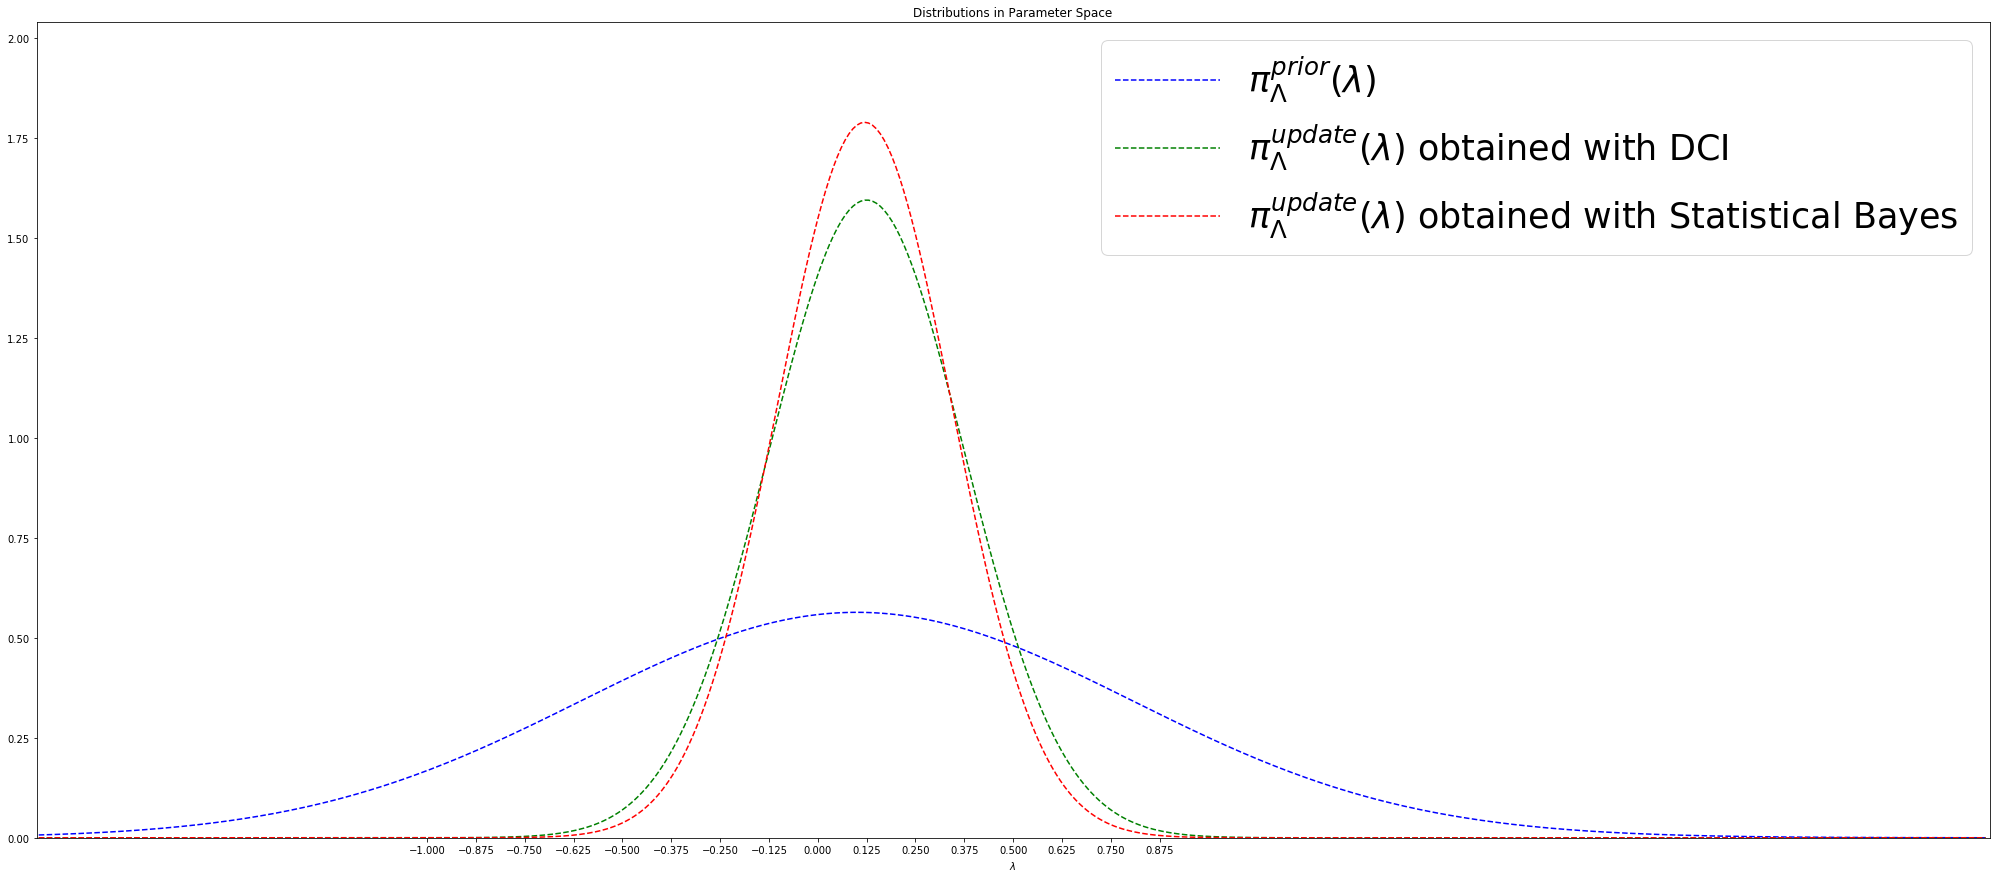
\includegraphics[scale=0.15]{param}

\textit{Distributions in parameter space from Example 1.}
\end{center}

\end{frame}


\begin{frame}

\begin{center} 
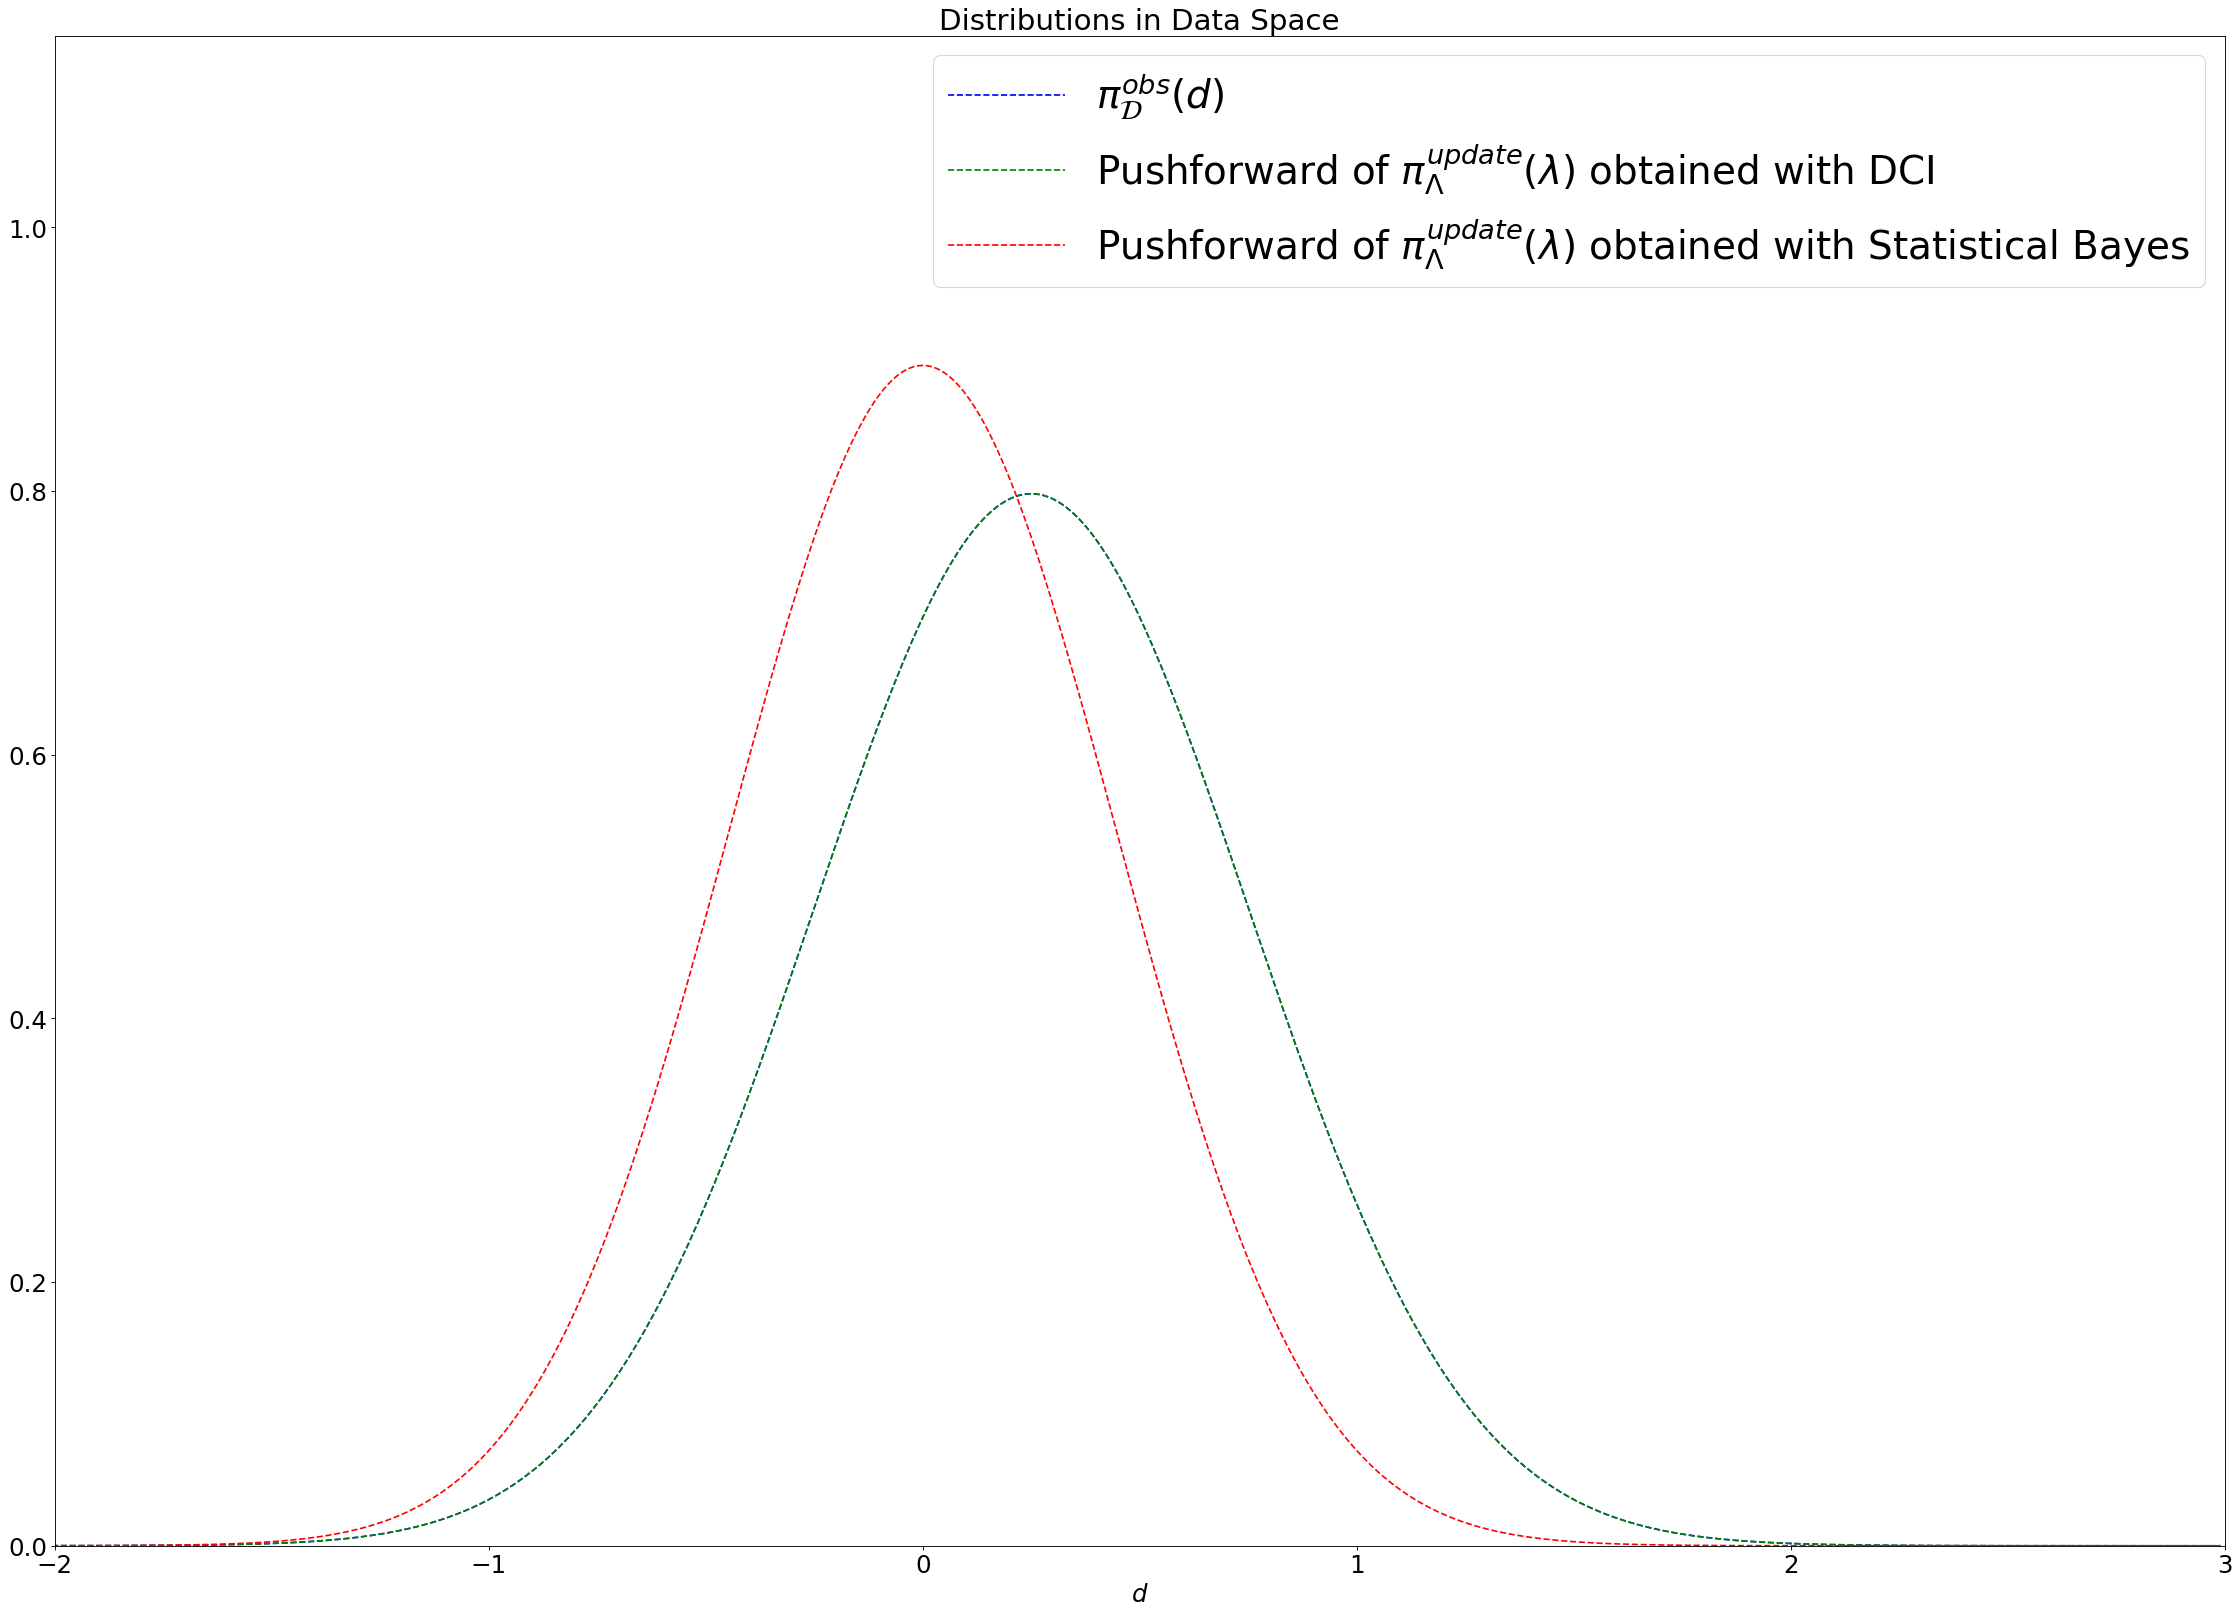
\includegraphics[scale=0.125]{data}

\textit{Distributions in data space from Example 1.}
\end{center}

\end{frame}


\begin{frame}

\begin{block}{Example 2. \footnotemark[1]}


\noindent  Let $f(\lambda)=2\lambda_1-\lambda_2$, $\lambda_\text{prior}=(0.1 \quad 0.2)^\top$, $C_\Lambda=\text{diag}[0.5,0.25],$ $d_\text{obs}=0.1$, and $C_\mathcal{D}=[0.25]$.

\vspace{0.25cm}

 With $N=2$ and $M=1$, for any $\lambda \in \Lambda$, $f(\lambda)=d=2\lambda_1-\lambda_2$. Since there is just a single $d_\text{obs}$, we have $0.1=2\lambda_1-\lambda_2$.

\vspace{.25cm}

We find $S$ is minimized by $\lambda^*_S=(7/50,19/100)$. 
Assuming that $\lambda_\text{prior}$ and $d_\text{obs}$ are the means of Gaussians with variances corresponding to the given covariance matrices, we have $\pi_\Lambda^\text{post} \sim \exp(-S(\lambda_S))$ with mean $\lambda_S^*$. Notice $f(\lambda^*_S)=9/100\neq d_\text{obs}$. 

\vspace{.25cm}
 
In the data-consistent formulation, we have 
$T$ minimized by $\lambda^*_T=(13/90,17/90)$. Notice $f(\lambda^*_T)=9/90=d_\text{obs}$. With Gaussian assumptions, we have $\pi_\Lambda^\text{post} \sim \exp(-T(\lambda))$ with mean $\lambda_T^*$. 

\end{block}


\footnotetext[1]{Wildey, T., Butler, T., Jakeman, J., Walsh, S.}
\end{frame}

\begin{frame}


\begin{figure} 
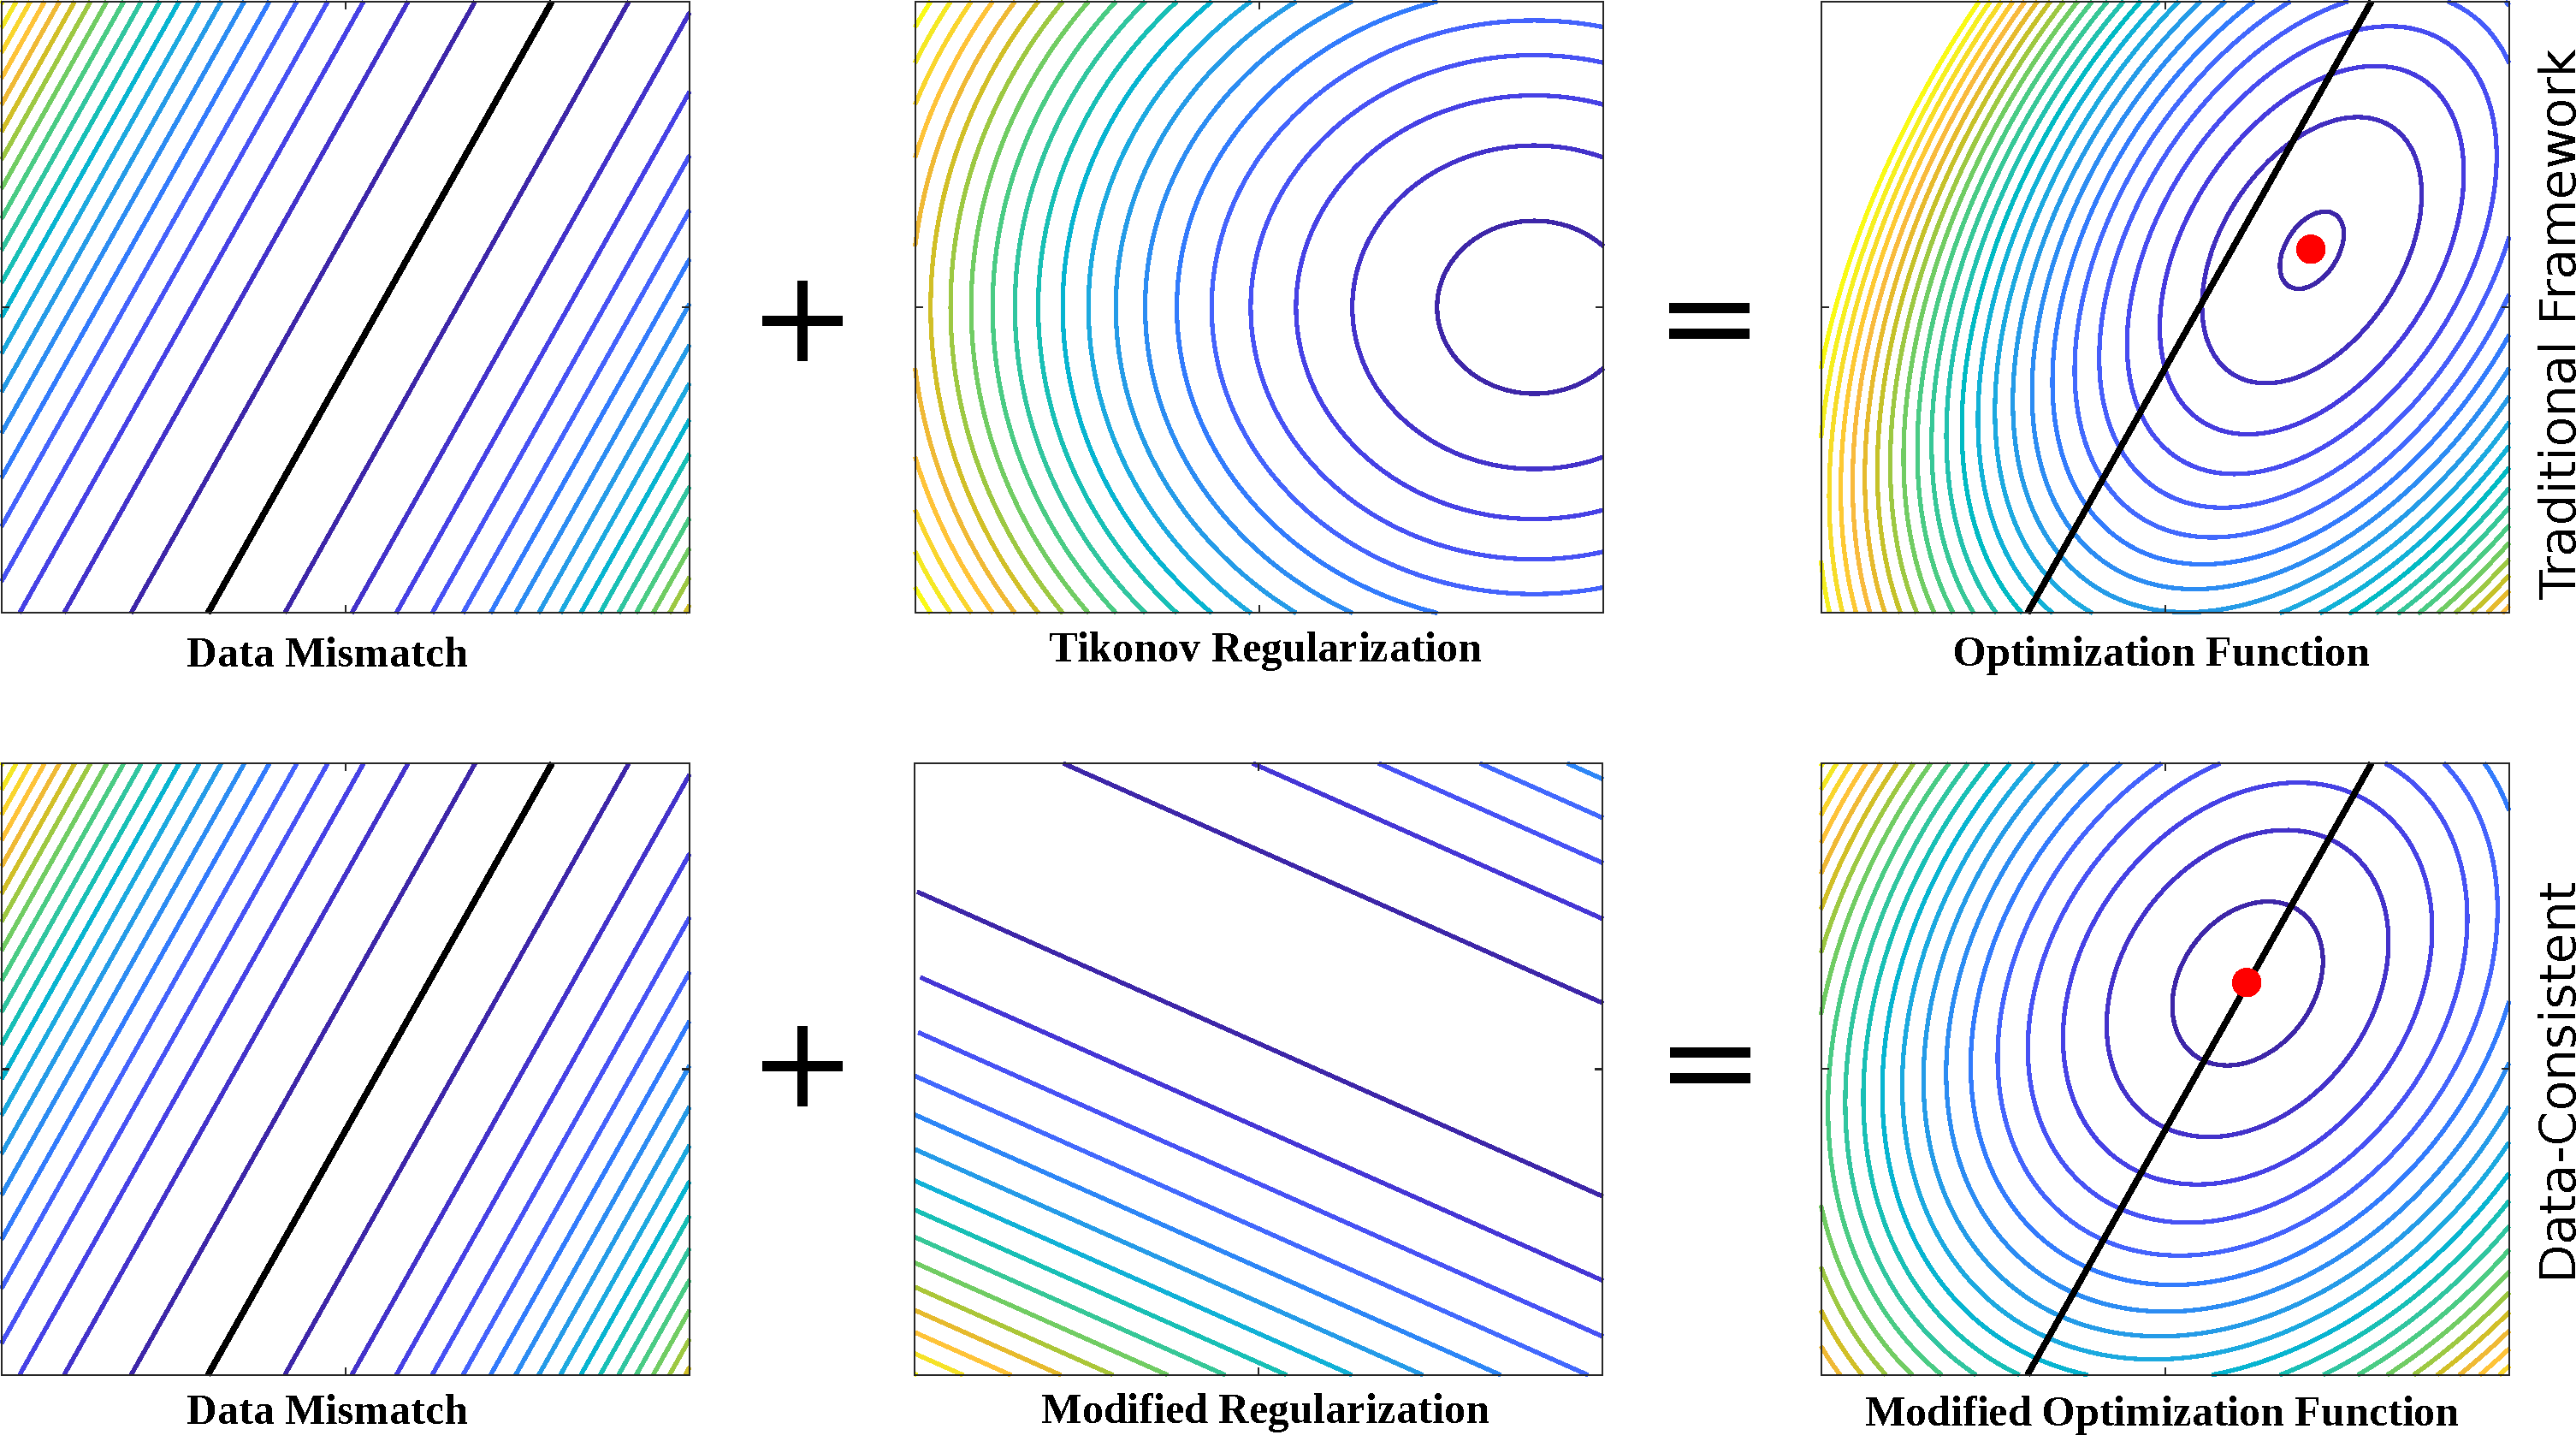
\includegraphics[scale=0.2]{Regularization-all-in-one.pdf}

This figure \footnotemark[1] shows the process of obtaining the statistical/classical Bayesian solution and data-consistent solution in Example 2.
\end{figure}

\footnotetext[1]{Wildey, T., Butler, T., Jakeman, J., Walsh, S.}

\end{frame}

% ------------------------------------------------
\subsection{Dimension Reduction}
% ------------------------------------------------

\begin{frame}

\begin{itemize}

	\item We consider functions $f: \Lambda \to \mathcal{D}$ where $\dim(\Lambda)=N$ is large and $\dim(\mathcal{D})=M$ is such that $M<N$ or $M<<N$.

\begin{itemize}
		\item Functions of interest may represent postprocessed quantities from the solution of complex physical models.
\end{itemize}

\item It is not often that every parameter has equal impact on function values -- usually some parameters matter more than others.

\item The dimension reduction techniques considered seek to explain outputs $f(\Lambda)$ in an \textit{active subspace} $\mathcal{A} \subset \Lambda$ for which $\dim(\A)<N.$

\begin{itemize}
\item Many common uses (e.g. statistics) of $f$ involve integration over $\Lambda$ and are subject to the "curse of dimensionality".
\item This forces the use of Monte Carlo or Quasi-Monte Carlo methods.
\item A lower-dimensional representation of $f$ may enable faster methods.
\end{itemize}


\end{itemize}


\end{frame}

\begin{frame}

\begin{itemize}

\item $\nabla f(\lambda)\in \Lambda$ is a column vector containing the $N$ partial derivatives of $f$, which for this discussion we assume exist, and are square integrable in $\Lambda$ equipped with some probability density that is positive everywhere in $\Lambda$ and 0 otherwise.

\begin{itemize}
		\item We consider $\pi_\Lambda^\text{prior}(\lambda)$, the density describing our prior state of knowledge, which we abbreviate as $\pi_\Lambda$.
\end{itemize}

\item For convenience, one transforms inputs $\lambda$ to the origin with some fixed variance, typically so that $\lambda\in [-1,1]^N$. We define

\end{itemize}

\begin{block}{Covariance in Gradient Space \footnotemark[1]}

\begin{equation} \label{eq:4}
W=\int_\Lambda \nabla f(\lambda) \nabla f(\lambda)^\top  \pi_\Lambda(\lambda) d\lambda,
\end{equation} 

\noindent which is an $N\times N$ symmetric positive semi-definite matrix.

\end{block}

%\footnotetext[1]{Constantine, Eftekkari, Wakin}
\footnotetext[1]{Constantine}


\end{frame}

\begin{frame}

\begin{itemize}



\item Interpreting $W$ as a certain covariance structure over $\Lambda$ leads one to the idea of computing the Singular Value Decomposition of $W$,

\begin{block}{Singular Value Decomposition (SVD) of $W$}

\begin{equation} \label{eq:5}
W=U\Sigma V^*,
\end{equation} 


\noindent where $U$ is $N \times N$ unitary, $\Sigma$ is $N \times N$ diagonal with the singular values of $W$ along its diagonal, and $V^*$ is $N \times N$ unitary.

\end{block}

\item We plot the singular values, $\{\sigma_i\}_{i=1}^n$ and seek a drop-off in magnitude between some pair of singular values, $\sigma_{j}$ and $\sigma_{j+1}$. The active subspace is the span of $u_1,\ldots,u_{j}$, which are the first $j$ columns of $U$, the left singular vectors of $W$. 


\end{itemize}

\end{frame}

\begin{frame}

\begin{itemize}

	\item For a point $\lambda \in \Lambda$, we define

\begin{block}{Projection into $\mathcal{A}$, \textit{active variables}}

\begin{equation} \label{eq:6}
  \mathcal{P}_\A(\lambda)=\sum_{i=1}^{j}\left( u_i^T \lambda\right)u_i, 
\end{equation}

\noindent which is the projection of $\lambda$ in the active directions of $f$.

\end{block}

\item We have arrived at the property that 

\begin{block}{Resolution of $f$ in $\mathcal{A}$}

\begin{equation} \label{eq:7}
f\left(\mathcal{P}_\A(\lambda)\right) \approx f(\lambda).
\end{equation}

\end{block}

\end{itemize}



\end{frame}


\begin{frame}

\begin{itemize}

\item Finding an active subspace requires forming an approximation to $W$ via Monte Carlo. Here we consider techniques in \footnotemark[1] \footnotemark[2].



\item We let $D_S=\{(\lambda_i,f(\lambda_i))\}_{i=1}^S$, which is a set of $S$ pairs of samples $\lambda_i \in \Lambda$ and their function values. 

\item One may use $D_S$ to approximate $\nabla f$. We denote each estimation to $\nabla f(\lambda_i) \approx \reallywidehat{\nabla f}(\lambda_i)$.

\item We form the $N \times S$ matrix $\tilde{W}$ (which we present as $\tilde{W}^\top$)

\end{itemize}

\begin{block}{Monte Carlo Approximation to $W$ \footnotemark[1]}


\begin{equation} \label{eq:4}
\tilde{W}^\top:=\begin{bmatrix}
\reallywidehat{\nabla f}(\lambda_1)
\cdot \cdot \cdot
\reallywidehat{\nabla f}(\lambda_S)\\
\end{bmatrix}.
\end{equation}  

\end{block}

\footnotetext[1]{Russi, T.M.}
\footnotetext[2]{Constantine, Eftekkari, Wakin}

\end{frame}


\begin{frame}

\begin{itemize}

	\item Forming the SVD of $\tilde{W}$, $\tilde{W}=\tilde{U}\tilde{\Sigma}\tilde{V}^*$, we search for a drop off in the magnitude of the singular values $\{\tilde{\sigma}_i\}_{i=1}^S$. Assuming such a drop off occurs for an index $j:1<j<S$, we have the $j$ corresponding left singular vectors,$ \tilde{u}_1,\ldots,\tilde{u}_{j}$.  
	
	\item Then we define

	\begin{block}{Monte Carlo approximation to $\A$}
	
	
	$$\A\left(f; D_S \right):=\text{span}\{\tilde{u}_1,\ldots,\tilde{u}_{j}\},$$ the active subspace of $f$ with respect to the samples $D_S$.
	
	\end{block}		

	\item For low dimensional $\A$, we may check $f(\mathcal{P}_\A(\lambda))\approx f(\lambda)$ in a \emph{sufficient summary plot}, where we plot active variables against function values.


\end{itemize}


\end{frame}

% ------------------------------------------------
\subsection{Derivative-Free Optimization (DFO)}
% ------------------------------------------------

\begin{frame}

\begin{itemize}

\item Many important physical systems possess turbulent or chaotic behavior.  

\item The physical state of the system $u(x,\lambda)$ and the corresponding parameter
to observable map $f(u(x,\lambda))$ may be modeled as a stochastic process, or as a deterministic function with additive or multiplicative noise.  

\begin{itemize}


\item In this setting, the efficient extraction of accurate gradients of $f$ in parameter space is a challenging undertaking, as popular techniques based on
linearization, including adjoint methods, are inaccurate \footnotemark[1] \footnotemark[2].  

\item The finite-difference approximation of $\nabla f_\Lambda$ 
involve $N=\text{dim}\Lambda$ 
additional, usually nonlinear model solves for the physical system state $u(x,\lambda_i + \delta \lambda_i)$, and may be greatly polluted by the noise in $f$.

\end{itemize}


\end{itemize}

\footnotetext[1]{Lea}
\footnotetext[2]{Qiqi}

\end{frame}

\begin{frame}

\begin{itemize}
 


\item We consider derivative-free optimization (DFO) algorithms suited for additive and multiplicative noise \footnotemark[1]. The technique only requires evaluations of the noisy model and random draws from a normal distribution.


\begin{itemize}


\item The method finds a new iterate by randomly perturbing the previous iterate in $\Lambda$.

\item Iterates are not allowed to stray much due to relatively small smoothing factors and step sizes. The smoothing factor and step size in the DF algorithms are of great importance to their convergence and termination. 

\item The smoothing factor and step size will depend on a scale factor of the $L_1$ Lipschitz constant of $f$. It is of interest to obtain estimates of $L_1$, which is not straightforward in a gradient-free setting. We refer to \footnotemark[2] \footnotemark[3] for Lipschitz constant learning.


\end{itemize}

\end{itemize}

\footnotetext[1]{Chen and Wild}
\footnotetext[2]{Jan-Peter Calliess}
\footnotetext[3]{Kvasov and Sergeyev}

\end{frame}


\begin{frame}

\begin{itemize}
	
	
	\item We consider the problem

\end{itemize}

\begin{block}{Optimization Under Additive Uncertainty \footnotemark[1]}
\begin{eqnarray} \label{eq:9}
\min_{\lambda \in \R^N} \quad \mathbb{E}\left[f(\lambda)+\nu (\lambda; \epsilon)\right],
\end{eqnarray} 


\begin{itemize}

\item where:

\begin{enumerate}[(i.)]

	\item $f: \R^N \to \R$ is convex;

	\item $\epsilon$ is a random variable with probability density $P(\epsilon)$;

	\item for all $\lambda$ the additive noise model $\nu$ is independent and identically distributed, has bounded variance $\sigma_a^2$, and is unbiased; i.e., $\mathbb{E}_\epsilon (\nu(\lambda;\epsilon))=0$.

\end{enumerate}


\end{itemize}


\end{block}

\footnotetext[1]{Chen and Wild}

\end{frame}


\begin{frame}

\begin{itemize}

	\item We consider algorithms such as \textit{STARS \footnotemark[1] (STep-size Approximation in Randomized Search)}, which: 

\begin{itemize}
		\item uses small perturbations in the domain $\Lambda=\R^N$ by the addition of a random vector with components drawn from a normal distribution to iterates $\lambda^{(k)}$; 
		\item computes the function value at the randomly perturbed point with additive or multiplicative noise drawn from a specified distribution; 
		\item and updates iterates using a Gaussian-smoothed finite-difference scheme for approximate gradient information in a gradient descent fashion. 

\end{itemize}

\end{itemize}

\footnotetext[1]{Chen and Wild}

\end{frame}




% ------------------------------------------------
\section{Research Questions}
% ------------------------------------------------


% ------------------------------------------------
\subsection{Data-Consistent Deregularization for Nonlinear $f$}
% ------------------------------------------------

\begin{frame}

\begin{itemize}
	
	% FIX THIS	
	
	\item For a general nonlinear map $f$, we must reformulate the deregularization which we recall for a linear map $f$ with matrix $A$ may be written

\begin{block}{Deregularization Term for Linear $f$}

\begin{equation} \label{eq:10}
\left|\left|C_A^{-1/2}(A\lambda-A\lambda_{\text{prior}})\right|\right|_2^2,
\end{equation} 

\noindent where $C_A=AC_\Lambda A^\top$. 

\end{block}

\item For a nonlinear $f$, we may expand $f$ linearly around some $\lambda \in \Lambda$ and write $f(\lambda)-f(\lambda_\text{prior})=A (\lambda-\lambda_\text{prior})$, where $A=\nabla f (\lambda)^\top$, which is an $N \times M$ matrix. In order to fully determine the form of \eqref{eq:10}, we must find $(f(\lambda)^\top C_\Lambda f(\lambda))^{-1}$.


\end{itemize}

\end{frame}

% ------------------------------------------------
\subsection{Impact of Noise on MAP Point and Updated Prior}
% ------------------------------------------------

\begin{frame}

\begin{itemize}

	\item The effects of noise on individual methods considered in this paper -- particularly: DCI, the deterministic optimization solution for SIPs, active subspaces, and DFO -- have been characterized to varying extents in corresponding literature. 
	
\begin{itemize}

		\item 	We investigate the impact of additive and multiplicative noise models in our framework, which may involve embedding the aforementioned methods in one another, performing them in series, or both.

\end{itemize}	


\item Formally, we investigate both sensitivity and stability of any proposed methods. 

\begin{itemize}

		\item Theoretically, this may involve using the individual sensitivity/stability analyses of certain methods while deriving new results when the methods are embedded or performed in series. 
		

\end{itemize}


\end{itemize}

\end{frame}

% ------------------------------------------------
\subsection{Learning and Sampling}
% ------------------------------------------------

\begin{frame}

\begin{itemize}

	\item We are interested in several problems that involve sampling $\Lambda$ and evaluating $f$ including solving the forward problem, finding an active subspace via Monte Carlo, and performing DFO.
	
	\begin{itemize}
	
		\item We are interested in comparing active subspaces obtained from sampling $f$ with few samples, or with samples generated from some other process, such as a DFO algorithm.
		
		\item 	Since many DFO algorithms use hyperparameters for step sizes and smoothing that depend on $L_1$, the literature \footnotemark[1] \footnotemark[2] contains attempts to learn Lipschitz constants from sampling alone.
	
	\end{itemize}


\end{itemize}

\footnotetext[1]{Jan-Peter Calliess}
\footnotetext[2]{Kvasov and Sergeyev}

\end{frame}


% ------------------------------------------------
\subsection{Using the Active Subspace}
% ------------------------------------------------



\begin{frame}

\begin{itemize}
	\item We are interested in investigating the effectiveness of only optimizing $f$ in its active variables.
	
	\item The most compelling approach we have observed is to modify the DFO algorithm discussed above to only take random walks in directions lying in $\A$.
	
	
	
	\begin{block}{Modified DFO Algorithm}
	Given the first $j$ singular unit vectors $u_1,\ldots,u_j$ corresponding to the SVD of $\hat{W}$, one may take $j$ draws from a specified normal distribution, which we denote with $s_i\sim N(\mu,\sigma^2)$, and form the random vector $v$ for the $k$-th step in a DFO algorithm as $v^{(k)}=\sum_{i=1}^js_iu_i$; we see that such a vector could be interpreted as a random walk in $\A$.
	
	\end{block}
	
	
	\item Other weighting schemes on the $u_i$'s could be considered, such as weights given by singular values.
	

	
\end{itemize}

\end{frame}


%\begin{frame}

%\begin{itemize}

%	\item We are generally interested in the representation and surrogates one may form with an active subspace.  
	
%\begin{itemize}


%	\item Depending on the quality and form of the resolution, one may (or may not) be able to discern the relation between $f$ and its active variables visually, by fitting a surrogate through the response surface and testing the fit, or both. 

% \end{itemize}	
	
%	\item Representing $f$ with a lower-dimensional surrogate may help with solving other problems of interest: we may be able to solve a forward problem at lower cost, or pose the convex objective function for solving an inverse problem using a surrogate.
	
% \end{itemize}


% \end{frame}


\begin{frame}

\begin{itemize}

	\item If the action of the map $f$ can be captured by a lower-dimensional representation, we may be able to more cheaply solve for the push-forward needed for DCI. 
	
	\item Research directions include: 
	
	\begin{itemize}
	

		\item comparing the cost of solving the forward problem with KDE for an $f$ defined in its full variables versus some surrogate for $f$ defined over $A$; 
		
		\item analyzing differences in MAP points obtained from updated densities in $\Lambda$ when the push-forward is obtained from its full variables versus only from active variables.

	\end{itemize}		

\end{itemize}


\end{frame}

% ------------------------------------------------
\subsection{Application: Callibrated Anomolous Diffusion in Tokamak Plasmas}
% ------------------------------------------------

\begin{frame}
\frametitle{Tokamak Geometry}
\vspace*{-.5in}

\centerline{ 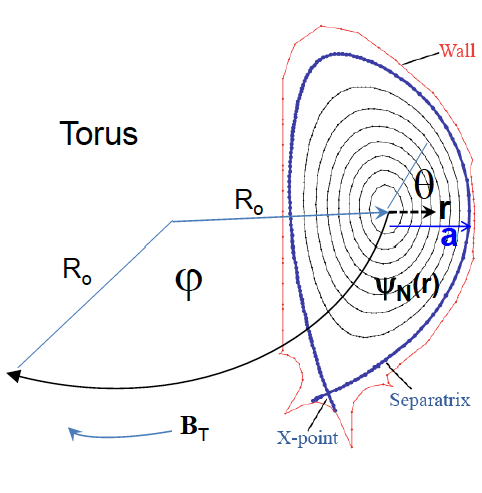
\includegraphics[height=.6 \textheight]{torus_coord.png}}

\centerline{Poloidal cross section at a constant toroidal angle}

\begin{itemize}
\item Normalized flux coordinate $\psi_N$: 0 at $r$, 1 at $\frac{r}{a}=1$.
\end{itemize}


\end{frame}

\begin{frame}
%\vspace*{-.25in}

\begin{block}{Transport in Tokamaks}
Transport in tokamak plasmas can be strongly driven by a combination of {\em neoclassical} effects
and plasma {\em microturbulence}.
\end{block}


%\frac {\partial f_{\alpha }}{\partial t}}+\mathbf {v} _{\alpha }\cdot {\frac {\partial f_{\alpha }}{\partial \mathbf {x} }}+{\frac {q_{\alpha }\mathbf {E} }{m_{\alpha }}}\cdot {\frac {\partial f_{\alpha }}{\partial \mathbf {v} }}=0,}

\centerline{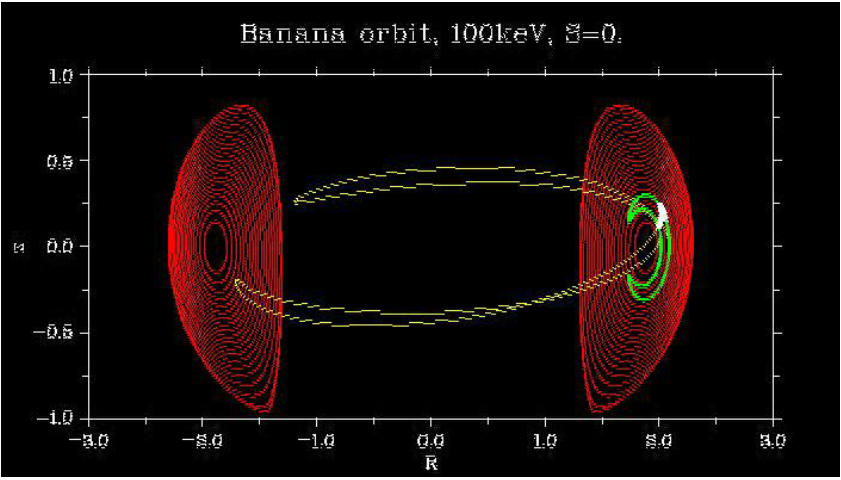
\includegraphics[width=.6\textwidth]{banana_orbit.png}}

\centerline{Neoclassical theory predicts complex particle motion}

\begin{itemize}
\item Neoclassical transport:  simplified Vlasov-Boltzman equation coupled with Maxwell's equations \footnotemark[1].
\end{itemize}

\footnotetext[1]{Wesson}

\end{frame}


\begin{frame}
	
Simulating the microturbulence in the plasma involves very expensive kinetic simulations, 
especially when simulating the plasma edge \footnotemark[1]. 

\begin{itemize}
	\item An alternate approach to simulate microturbulence is by fitting an anomalous diffusion model.
	\begin{itemize} 
	\item Fit using  experimental data
 	\item Direct Numerical Simulation(DNS) approach: Fit using high-fidelity simulation data.
 	\item Deterministic efforts in this setting include \footnotemark[2]. 
\end{itemize}
\item This approach is similar to common modeling techniques in  parameterizing micro-scale
effects in macro/meso-scale systems.(e.g. turbulence models, sub-grid models) 

 \end{itemize}
 
%\centerline{ 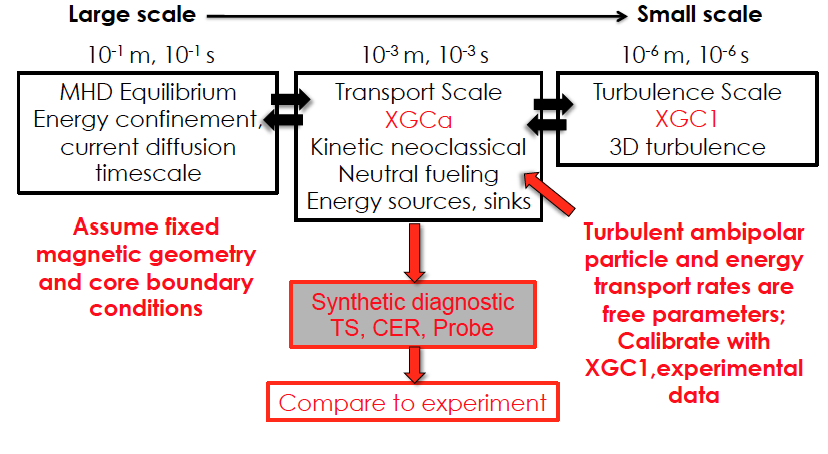
\includegraphics[height=.4\textheight]{xgca_calibrate.png}}

\footnotetext[1]{S. Ku and R. Hager and C.S. Chang and J.M. Kwon and S.E. Parker}
\footnotetext[2]{Battaglia et al}

\end{frame}
 
 \begin{frame}
 
 \centerline{ 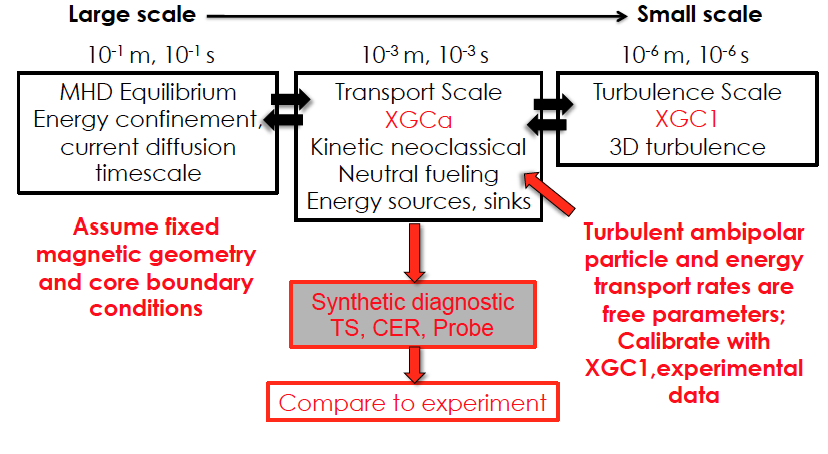
\includegraphics[height=.6\textheight]{xgca_calibrate.png}}
 
 \begin{block}{Research Question}
 We propose to investigate the data-consistent calibration of an anomalous diffusion model in an axisymmetric setting (XGCa) to high-fidelity experimental or simulation data (XGC1) \footnotemark[1].
\end{block}
	

\footnotetext[1]{S. Ku and R. Hager and C.S. Chang and J.M. Kwon and S.E. Parker}
\end{frame}

% ------------------------------------------------
\subsection{Application: Magnetic Equilibria in Tokamaks}
% ------------------------------------------------

\begin{frame}

	\begin{itemize}
	

	\item In dimensionless coordinates, the axisymmetric  Grad-Shafronov equation is given by
	
	\begin{block}{The Grad-Shafronov Equation \footnotemark[1]}

\begin{equation}
r\frac{\partial}{\partial r} \left( \frac{1}{r} \frac{\partial\psi_n}{\partial r} \right) + \frac{\partial^2 \psi_n}{\partial z^2} = -\frac{\alpha^2}{2} \frac{d f^2}{d \psi_n} - r^2\alpha^2 \frac{dp}{d\psi_n}.
\end{equation}

	\end{block}


	\item In equilibrium fitting to experimental data \footnotemark[2], $p$ and $f^2$ are expanded as basis functions (usually polynomials) in $\psi_n$, with the extra constraint that $p$ and $f^2$ vanish at the boundary.

\begin{itemize}
\item DCI problem: Findi the updated PDF of the uncertain parameters in the expansions of $p$ and $f^2$. 
\item Updated  PDF icrucial to prediction of plasma profiles % (e.g. ion/electron density or temperature) 
and transport as these properties.
%are extremely sensitive to perturbations
%n the magnetic equilibrium, especially in the edge.

\end{itemize}

\end{itemize}

\footnotetext[1]{Takeda, T. and Tokuda, S.}
\footnotetext[2]{Lao et al}

\end{frame}


% ------------------------------------------------
\section{Preliminary Results and Research Plan}
% ------------------------------------------------


% ------------------------------------------------
\subsection{Data-Consistent Deregularization for Nonlinear $f$}
% ------------------------------------------------

\begin{frame}


\begin{itemize}

	\item We must consider ways to express the deregularization for nonlinear $f$. This is a theoretical task which will require a closer literature review and heavy collaboration with advisers.

	\item Ideas to explore may include ways in which the active subspace of $f$ could lead to more easily obtained linearizations around particular points in $\Lambda$
	
	\item We also must consider more general surrogate modeling. As we will observe, the $f$ as defined in Example 3 is globally quadratic with respect to its active subspace, and won't permit a global linearization. We may consider, however, a local linearization at various points on the response surface $f(\mathcal{P}_A(\lambda))$ which may be acceptable, particularly near 0.

\end{itemize}


\end{frame}

% ------------------------------------------------
\subsection{Impact of Noise on MAP Point and Updated Prior}
% ------------------------------------------------

\begin{frame}

\begin{itemize}

	\item We have performed several numerical experiments in which $f$ with additive noise is minimized with DFO at the same time that the active subspace is formed. For comparison, we have also performed numerical experiments in which $f$ with additive noise is minimized via DFO with no active subspace analysis, and likewise we have searched for the active subspace of $f$ using random points in $\Lambda$.
	


	\item The first concrete research step to obtain experimental evidence of noise effects will be increasing the noise level until results no longer match expectations. Rigorous characterization must follow.
	
	\item With an understanding of how error impacts DFO and active subspaces, we can consider the impact of noise on MAP points and updated priors.


\end{itemize}

\end{frame}

% ------------------------------------------------
\subsection{Learning and Sampling}
% ------------------------------------------------

\begin{frame}

\begin{block}{Example 3.}


Let $\Lambda=[-1,1]^{11}$ and define $$f(\lambda)=\sum_{i=0}^{10} 2^{(-1)^i i}\lambda_i^2+\epsilon(\lambda),$$ where $\epsilon(\lambda)$ is a draw of additive noise corresponding to the input $\lambda$; here, we take draws of $\epsilon$ of order $10^{-4}$. We see that $\mathcal{D}=[0,2^{10}]$ and $N=11$, $M=1$. Note that the minimimum of $f$ is given by $0 \in \Lambda$. Here, as $i$ increases, terms in $f$ become either more important or less important, depending on whether $i$ is even or odd.

\end{block}

\end{frame}

\begin{frame}

\begin{center}

 
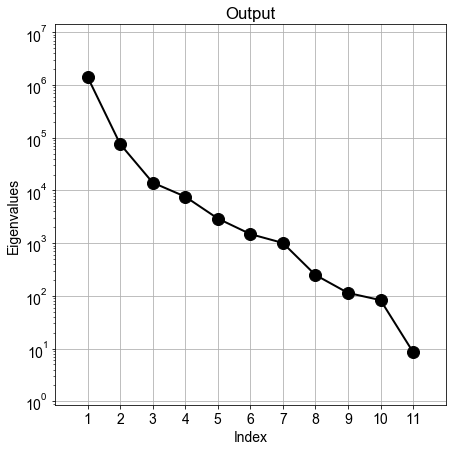
\includegraphics[scale=0.3]{eigs.png} 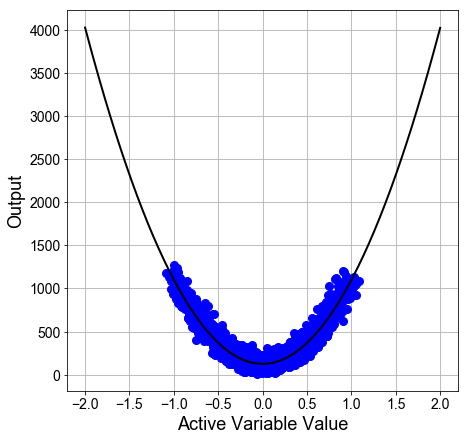
\includegraphics[scale=0.3]{surr.png}

Left: A plot of the eigenvalues of the matrix $\hat{W}$ formed from 1000 Monte Carlo samples in $\Lambda$. We see one dominant eigenvalue on the order of $10^6$. Right: A sufficient summary plot where all 1000 samples are projected into $\A$ and plotted against their function values; a quadratic surrogate fits the projected data with $R^2\approx 0.9$.

\end{center}



\end{frame}

\begin{frame}

\begin{center}

 
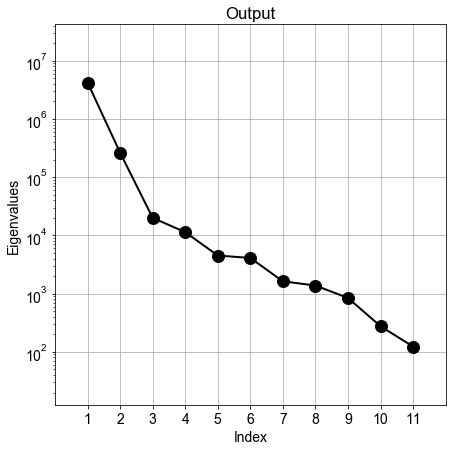
\includegraphics[scale=0.3]{DFO_eigs.png} 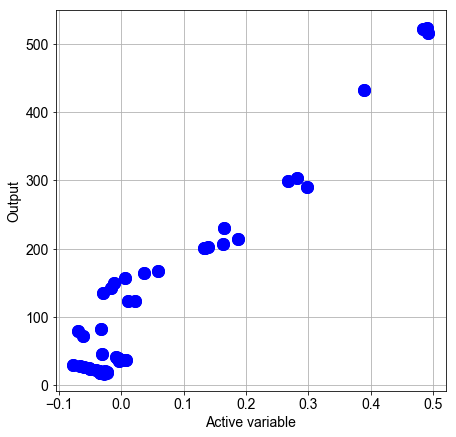
\includegraphics[scale=0.3]{DFO_suffsum.png}

Left: A plot of the eigenvalues of the matrix $\hat{W}$ formed from using 100 DFO iterates as samples in $\Lambda$. We again see one dominant eigenvalue between orders $10^6$ and $10^7$. Right: A sufficient summary plot where all 100 samples are projected into $\A$ and plotted against their function values.

\end{center}



\end{frame}

% ------------------------------------------------
\subsection{Using the Active Subspace}
% ------------------------------------------------

\begin{frame}

\begin{itemize}

	\item We are generally interested in using the active subspace of a function whenever it may reduce
computational expense while maintaining a representations that does not deviate too far from the true action of $f$. 

\begin{itemize}


	\item Here we consider the effectiveness of DFO performed on $f$ from Example 3 using 500 iterations of unmodified STARS versus a scheme that blends STARS and active subspace analysis using only 150 iterations.
	
	

\end{itemize}


\end{itemize}


\end{frame}

\begin{frame}


\begin{center}

 
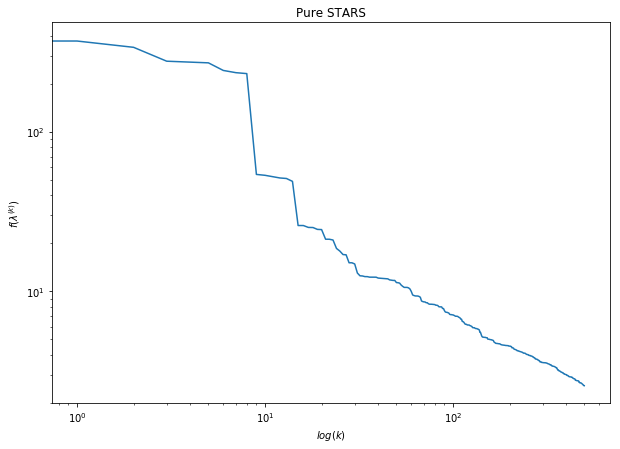
\includegraphics[scale=0.25]{pure_stars.png} 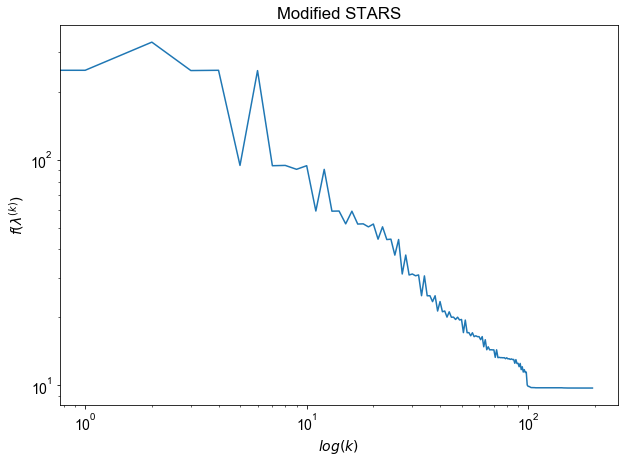
\includegraphics[scale=0.25]{mod_stars.png}

Left: A log-log plot of the number of iterations (500) versus their function values in STARS. Right: A log-log plot of the number of iterations (150) versus their functions values in modified STARS.

\end{center}


\end{frame}


% ------------------------------------------------
\subsection{From Model Problems to Fusion Applications}
% ------------------------------------------------

\begin{frame}

We propose to investigate the approximate solution of data-consistent inverse problems via optimization approaches.

\begin{block}{Derivative Free Optimization}
\begin{itemize}
	\item Initial model functions + noise
        \item  data consistent inversion of a subgrid LES model for isotropic turbulent flow.  
        \item data consistent inversion of an anomalous diffusion model for gyrokinetic turbulence in XGCa.
        \end{itemize}
\end{block}

\begin{block}{Gradient-based methods}
\begin{itemize}
	%\item In the case of models where $\lambda$-gradients are available and not of suspect quality, we will transition from 
	\item an approximate DCI for a model elliptic problem with a parameterized forcing function, with parameter gradients obtained via adjoint methods.  
	\item Data-consistent MHD equilibria (Grad-Shafronov)
\end{itemize}
\end{block}


\end{frame}

% ------------------------------------------------
\subsection{Software Dissemination}
% ------------------------------------------------


\begin{frame}

\begin{itemize}

	\item Currently, only some of the software used to produce results in this paper are publicly available on GitHub.com. 
	
	\item Some of the algorithms used here and other algorithms that are of interest are within open-source packages available online \footnotemark[1] \footnotemark[2]. 
	
	\item Other schemes considered here make modifications to given algorithms and remain under development. A major goal of this thesis proposal will be producing well-documented, open-source software complete with python Jupyter Notebooks containing illustrative, replicable examples.


\end{itemize}

\footnotetext[1]{T. Butler and J. Jakeman and T. Wildey}
\footnotetext[2]{Constantine}

\end{frame}



% ------------------------------------------------
\section{Timeline}
% ------------------------------------------------
\begin{frame}

We outline a rough timeline for the remaining 2 years in a 5.5 year plan.

\begin{itemize}
\small

\item Clean existing algorithms and examples, generate richer research results related to DFO and active subspaces, and build a model inverse problem for investigation. (Dec 2018/Jan 2019)

\item On RA for Spring 2019. (Jan 2019-May 2019)

\item Write and present MS-level results. (Feb/Mar 2019)

\item Work on theoretical formulation of deregularization for nonlinear $f$. Work on generating notebooks and examples. (Ongoing/Spring and Summer 2019)

\item Summer research; begin writing thesis; summer school/internship/conferences. (Jun/Jul/Aug 2019)

\item Fall 2019 - Writing phase, revisions. 

\item Spring 2020 - Final revisions, software, documentation.

\item Summer 2020 Internship/collaborations, publishing, formatting.

\item Defend thesis Summer 2020 or early Fall 2020.


\end{itemize}


\end{frame}



% ------------------------------------------------

\section{References}
% ------------------------------------------------
\begin{frame}[allowframebreaks]

%%%%%%%%%%%%%% References %%%%%%%%%%%%%%%%%%%%%%%%%
\begin{thebibliography}{65}

\tiny

\bibitem{battaglia} Battaglia, D. J.  and Burrell, K. H.  and Chang, C. S.  and Ku, S.  and deGrassie, J. S.  and Grierson, B. A. ``Kinetic neoclassical transport in the H-mode pedestal." Physics of Plasmas,Volume 21, No. 7. 2014.


\bibitem{BJW18a} T. Butler and J. Jakeman and T. Wildey.
``Combining Push-Forward Measures and Bayes' Rule to Construct Consistent Solutions to Stochastic Inverse Problems." SIAM Journal on Scientific Computing, Volume 40, No. 2, pp. A984-A1011, 2018.

\bibitem{Calliess} Jan-Peter Calliess. ``Lipschitz optimisation for Lipschitz interpolation." In 2017 American Control Conference (ACC 2017), Seattle, WA, USA, May 2017.

\bibitem{CW} Chen and Wild. ``Randomized Derivative-Free Optimization of Noisy Convex Functions." Funded by the Department of Energy. 2015.

\bibitem{Constantine2015} Constantine, Paul G. ``Active Subspaces: Emerging Ideas for Dimension Reduction in Parameter Studies." SIAM, 2015.

\bibitem{ConstantineMC} Constantine, Eftekhari, Wakin. ``Computing Active Subspaces Efficiently with Gradient Sketching." Conference paper, 2015 IEEE 6th International Workshop on Computational Advances in Multi-Sensor Adaptive Processing (CAMSAP).


\bibitem{KS} Kvasov and Sergeyev. ``Lipschitz gradients for global optimization in a one-point-based partitioning scheme." Journal of Computational and Applied Mathematics. Volume 236, Issue 16, pp. 4042-4054. 2012.

\bibitem{KU_TOTALF} S. Ku and R. Hager and C.S. Chang and J.M. Kwon and S.E. Parker. ``A new hybrid-Lagrangian numerical scheme for gyrokinetic simulation of tokamak edge plasma." Journal of Computational Physics, Volume 315, pp. 467-475. 2016.

\bibitem{Lao85} Lao, L.L, St. John, H, R.D. Stambaugh, A.G. Kellman, and Pfeiffer, W.,``Reconstruction of current profile parameters and plasma shapes in tokamaks'', Nuclear Fusion, Volume 25,No. 11,pp. 1611,1985.

\bibitem{lea2000} Lea, Daniel J. and Allen, Myles R. and Haine, Thomas W. N. ``Sensitivity analysis of the climate of a chaotic system." Tellus A, Volume 52, No. 5, pp. 523-532. 2000.



\bibitem{Russi} Russi, Trent M. ``Uncertainty Quantification with Experimental Data and Complex System Models." Dissertation, University of California Berkeley. 2010.

\bibitem{Smith}  Smith, Ralph.``Uncertainty Quantification: Theory, Implementation, and Applications.” SIAM, 2013.

\bibitem{Stuart} Stuart, Andrew. ``Inverse problems: A Bayesian perspective." Acta Numerica, volume 19, pp. 451-559. 2010.



\bibitem{Tarantola} Tarantola, Albert. ``Inverse Problem Theory and Methods for Model Parameter Estimation." SIAM. 2005.

\bibitem{Takeda91} Takeda, T. and Tokuda S.,``Computation of MHD equilibrium of tokamak plasma'',
Journal of Computational Physics,93,1,1 - 107,1991.

\bibitem{Qiqi2014} Qiqi Wang and Rui Hu and Patrick Blonigan. ``Least Squares Shadowing sensitivity analysis of chaotic limit cycle oscillations." Journal of Computational Physics, Volume 267, pp. 210-224. 2014.


\bibitem{Wesson} Wesson, J. ``Tokamaks." ``Oxford University Press, 4th edition." 2011.

\bibitem{wildeyprez} Wildey, T., Butler, T., Jakeman, J., Walsh, S. " A Consistent Bayesian Approach for Stochastic Inverse Problems Based on Push-forward Measures." SAND2017-3436PE. 2017.


\end{thebibliography}






\end{frame}







\end{document}

